\documentclass{acm_proc_article-sp}

\usepackage[greek, english]{babel}
\usepackage[utf8]{inputenc}

\usepackage[T1]{fontenc}

\usepackage[activate=compatibility]{microtype}

% autoref command
\usepackage[pdftex,urlcolor=black,colorlinks=true,linkcolor=black,citecolor=black]{hyperref}
\def\sectionautorefname{Section}
\def\subsectionautorefname{Subsection}
\def\subfloatautorefname{Subfigure}

\usepackage[lofdepth,lotdepth]{subfig}

\usepackage{enumitem}

\usepackage{mathtools}

% give emph a normal fontsize
\let\oldemph\emph
\renewcommand{\emph}[1]{\oldemph{\fontsize{9}{9}\selectfont #1}}

% more readable footnote layout
\renewcommand{\footnotesize}{\fontsize{8pt}{10pt}}
\setlength{\footnotesep}{.5cm}

% todo macro
\usepackage{color}
\newcommand{\todo}[1]{\noindent\textcolor{red}{{\bf \{TODO}: #1{\bf \}}}}

% listings and Verbatim environment
\usepackage{fancyvrb}
\usepackage{relsize}
\usepackage{listings}
\usepackage{verbatim}
\newcommand{\defaultlistingsize}{\fontsize{8pt}{9.5pt}}
\newcommand{\inlinelistingsize}{\fontsize{8pt}{11pt}}
\newcommand{\smalllistingsize}{\fontsize{7.5pt}{9.5pt}}
\newcommand{\listingsize}{\defaultlistingsize}
\RecustomVerbatimCommand{\Verb}{Verb}{fontsize=\inlinelistingsize}
\RecustomVerbatimEnvironment{Verbatim}{Verbatim}{fontsize=\defaultlistingsize}
\lstset{frame=lines,captionpos=b,numberbychapter=false,escapechar=§,
        aboveskip=0.5em,belowskip=0em,abovecaptionskip=0em,belowcaptionskip=0em,
framexbottommargin=-1em,
        basicstyle=\ttfamily\listingsize\selectfont}

% use Courier from this point onward
\let\oldttdefault\ttdefault
\renewcommand{\ttdefault}{pcr}
\let\oldurl\url
\renewcommand{\url}[1]{\inlinelistingsize\oldurl{#1}}

% linewrap symbol
\definecolor{grey}{RGB}{130,130,130}
\newcommand{\linewrap}{\raisebox{-.6ex}{\textcolor{grey}{$\hookleftarrow$}}}

% more pleasing quote environment
\usepackage{tikz}
\newcommand*{\openquote}{\tikz[remember picture,overlay,xshift=-7pt,yshift=1pt]
     \node (OQ) {\fontfamily{fxl}\fontsize{16}{16}\selectfont``};\kern0pt}
\newcommand*{\closequote}{\tikz[remember picture,overlay,xshift=2pt,yshift=-4.5pt]
     \node (CQ) {\fontfamily{fxl}\fontsize{16}{16}\selectfont''};}
\renewenvironment{quote}%
{\setlength{\parindent}{1cm}\par\openquote}
{\closequote\vspace{-4.5pt}
}

\begin{document}

\title{Fixing the Web one page at a time,\\ or actually implementing xkcd \#37}

\numberofauthors{2}
\author{
\alignauthor
Thomas Steiner\\
	\affaddr{Universitat Polit\`{e}cnica}\\
	\affaddr{de Catalunya}\\
	\affaddr{Department LSI}\\
	\affaddr{08034 Barcelona, Spain}\\
	\email{tsteiner@lsi.upc.edu}
\alignauthor
Ruben Verborgh\\
	\affaddr{Ghent University -- IBBT, ELIS}\\
	\affaddr{Multimedia Lab}\\
	\affaddr{Gaston Crommenlaan 8/201}\\
	\affaddr{9050 Ghent, Belgium}\\
	\email{ruben.verborgh@ugent.be}
}
\maketitle

\begin{abstract}
\begin{figure}[h!]
\centering
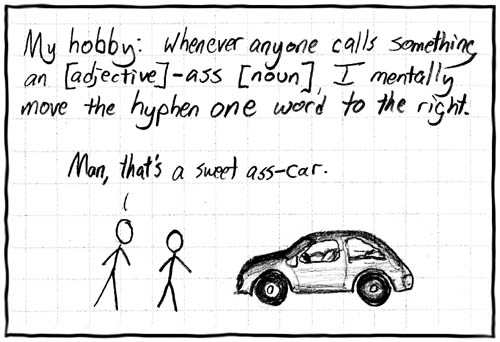
\includegraphics[width=\columnwidth]{hyphen.jpg}
\caption{xkcd \#37 -- I do this constantly \cite{xkcd37}.}
\label{fig:xkcd37}
\end{figure}
\end{abstract}

%\category{H.3.4}{Information Systems}{Information Storage and Retrieval}[World Wide Web]
%\category{H.3.5}{Online Information Services}{Web-based services}

%\keywords{}

\section{Introduction}
Albeit famous exceptions exist in form of Wikis,
the Web today is still mostly a~read-only experience.
This leaves the Web content consumer exposed to all sorts of typographic cruelties,
such as representing the ellipsis character '\ldots' with three single full stops ``...'',
incorrect usage of a \linebreak % !!!!!!!!! IMPORTANT !!!!!!!!!
normal space where a~non-breaking space would be preferred
and even omission of the Oxford comma...
While fighting the cause, sloppy authors, is like a~fight against wind mills
and certainly impossible to realize on Web scale,
fighting the symptoms is a~realistic option.
Using client-side work-arounds, the Web can actually be fixed one page at a~time.
In this paper, we show how using browser extensions, part of speech tagging,
and JavaScript DOM event listeners,
the Web can be made a~place worth wasting ones lives.

\section{Typographic Annoyances}
In this Section, we shamelessly adapt, copy,
and paste Wikipedia definitions for common typographic annoyances.

\textbf{Ellipsis character:} Ellipsis (plural ellipses; from the Ancient Greek:
\greektext élleiyis, % ἔλλειψις  % !!!!!!!!! IMPORTANT !!!!!!!!!
\latintext élleipsis, ``omission'' or ``falling short'')
is a~series of marks that usually indicate an intentional omission of a~word,
sentence, or whole section from the original text being quoted.
An ellipsis can also be used to indicate an unfinished thought or,
at the end of a~sentence, a~trailing off into silence (aposiopesis).
It can also be used at the end of a~sentence to emphasize a~statement.
When placed at the beginning or end of a~sentence,
the ellipsis can also inspire a~feeling of melancholy or longing.
The ellipsis calls for a~slight pause in speech or any other form of text,
but it is incorrect to use ellipses solely to indicate a~pause in speech.
The ellipsis character is commonly incorrectly represented
by three full stops in a~row due to the lack of a~designated key on standard computer keyboards.

\textbf{Oxford comma:} The Oxford comma is the comma used immediately before a coordinating conjunction (usually ``and'' or ``or'',
and sometimes ``nor'') preceding the final item in a~list of three or more items.
For example, a~list of three countries can be punctuated as either
``Portugal, Spain, and France'' (with the Oxford comma) or as
``Portugal, Spain and France'' (without the Oxford comma).
Opinions vary among writers and editors on the usage or avoidance of the serial comma.
In American English, the serial comma is standard usage in non-journalistic writing that follows the Chicago Manual of Style.
Journalists, however, usually follow the AP Stylebook, which advises against it,
albeit the AP Stylebook errs here.
There is no known valid excuse for not using the Oxford comma.

\textbf{Non-breaking space:} In computer-based text processing and digital typesetting,
a~non-breaking space or no-break space (NBSP) is a~variant of the space character that prevents an automatic line break (line wrap) at its position.
Text-processing software typically assumes that an automatic line break may be inserted anywhere a~space
character occurs;
a~non-breaking space prevents this from happening (provided the software recognizes the character).
For example, if the text ``100 km'' will not quite fit at the end of a~line,
the software may insert a~line break between ``100'' and ``km''.
To avoid this undesirable behaviour, the editor may choose to use a~non-breaking space between ``100'' and ``km''.
This guarantees that the text ``100 km'' will not be broken:
if it does not fit at the end of a~line
it is moved in its entirety to the next line.
Due to its non-presence on standard keyboards,
the non-breaking space typically gets represented by a~normal white space character.

\section{Further Use Cases}
In this Section, we present further use cases where client-side fixing of Web pages can be considered useful.

\textbf{xkcd \#37:} The Web comic xkcd in its episode \#37 proposes the mental experiment of shifting the hyphen in word combinations of the form \mbox{``[adjective]-ass [noun]''} one word to the right,
so that the resulting word combination reads \mbox{``[adjective] ass-[noun]''}.

\textbf{Emoticons:} An emoticon is a pictorial representation of a~facial expression using punctuation marks and letters,
usually written to express a person's mood.
Emoticons are often used to alert a responder to the tenor or temper of a statement,
and can change and improve interpretation of plain text.
Not emoticon-aware software unfortunately still has the tendency to break lines in the middle of an emoticon \texttt{:-} \linebreak % !!!!!!!!! IMPORTANT !!!!!!!!!
\texttt{(}. This can be avoided by the dynamic client-side insertion of non-breaking spaces.

\section{Implementation}
In this Section, we detail the implementation and underlying technologies used.

\subsection{Part-of-Speech Tagging}
A simple definition of part-of-speech tagging (POS) is the process of identifying words in a text as nouns, verbs, adjectives, adverbs, etc., based on both their definition, as well as their context.
Our processing chain supports part-of-speech tagging via an open source JavaScript library called jspos\footnote{\url{http://code.google.com/p/jspos/}},
eventually based on Eric Brill's POS tagger~\cite{brill1992simple}.

\subsection{Browser Extensions}
Browser extensions are small software programs that users can install to enrich their browsing experience with Web browsers.
They are written using a combination of standard Web technologies, such as HTML, JavaScript, and CSS.
There are several types of extensions; for this paper we focus on extensions based on so-called \emph{content scripts}.
Content scripts are JavaScript programs that run in the context of Web pages via dynamic code injection.
By using the standard Document Object Model (DOM), they can modify details of Web pages.

\subsection{Using Google Spreadsheets with JSON-P}
% Responsible: Tom
\cite{jsonp2009}

\subsection{Getting \todo{Manipulating?} All Text Nodes}
\label{subsec:textnodes}
% Responsible: Tom
http://jsperf.com/

\subsection{Listening on DOM Changes}
% Responsible: Ruben
The functionality so far only enables us to fix the static Web, \emph{i.e.}, Web pages whose content remains unchanged during their entire lifetime.
However, an important share of modern Web pages makes use of dynamically retrieved information, for example with AJAX technologies.
This means that a~single text node manipulation cycle after the initial page has been loaded is insufficient.

Instead, we have to dynamically react on page changes by listening to DOM events~\cite{w3cevents2011}.
Therefore, we add listeners for the \Verb!DOMCharacterDataModified! event, which occurs if the data of a~text node is changed.
Additionally, we monitor the \Verb!DOMSubtreeModified! event to watch when new elements are added to the DOM.
If this is the case, we also inspect their contents for possible replacements.

Finally, the \Verb!title! element deserves special attention.
While it resides in the \Verb!head! element and thus out of the visible part of the DOM~(in the \Verb!body! element),
browsers usually display the title in a~prominent place.
For that reason, title changes are separately monitored by the \Verb!DOMSubtreeModified! event.

\subsection{Security Considerations}
% Responsible: Ruben

\begin{lstlisting}[caption=Pseudocode illustrating the browser extension's functionality., label=code:xkcd, float=h, escapechar=§, belowskip=-1em]
// Initial processing
for all text nodes of DOM tree as text node
  processRules(text node)
end for  

// DOMNodeInserted Event Listener
on DOM node inserted (new node)
  for all text nodes of new node as text node
    processRules(text node)
  end for  
end on DOM node inserted

// Helper function
function processRules(text node)
  for all rules as rule
    if rule is regular expression rule
      apply rule to text node
    else if rule is part-of-speech tagging rule
      apply part-of-speech tagging to text node
      apply rule to parsed text node
    end if
  end for
end function  
\end{lstlisting} 

\section{Acknowledgments}
None. The world is to acknowledge us for this work.

% back to normal size Computer Modern for URLs in bibliography
\let\ttdefault\oldttdefault
\let\url\oldurl

\bibliographystyle{abbrv}
\bibliography{www2012}

\balancecolumns
\end{document}